\section{Task Set}
Here we discuss how the road networks that made up the task set were created, and how they were selected.

The size of the task set was based on two criteria. First, there needed to be enough tasks to get a good idea about performance. Second, the experiment was confined to be between 10-15 minutes based on the budget for the experiment, and also how long a participant could attend to tasks like this without losing interest. Using this criteria we decided to use around 40 tasks.

Experiment data was generated by generating random networks within the following bounds: N = [8,35] (based on computational concerns), p_trans=[0.0,1.0]. The starting position of the unmanned delivery truck (UDT) and the motorcycle gang (MG), and delivery destination were randomly selected from the available nodes.

Each road network was created by selecting a value for N in the given range, then randomly selecting a method from \emph{Watts-Strogatz}, \emph{expected degree}, \emph{Erd\:{o}s-R\`{e}ni} specifying N and E (number of edges), \emph{static scale free}. All graphs were required to be fully connected. A total of 500 networks were generated using this method, and \xQ{} and \xO{} were calculated for each one. Figure~\ref{fig:experiment_data} shows the full data set on the top, and the experiment task set on the bottom.

\begin{figure}[tbp]
    \centering
    \begin{subfigure}[b]{0.80\linewidth}
        \centering
        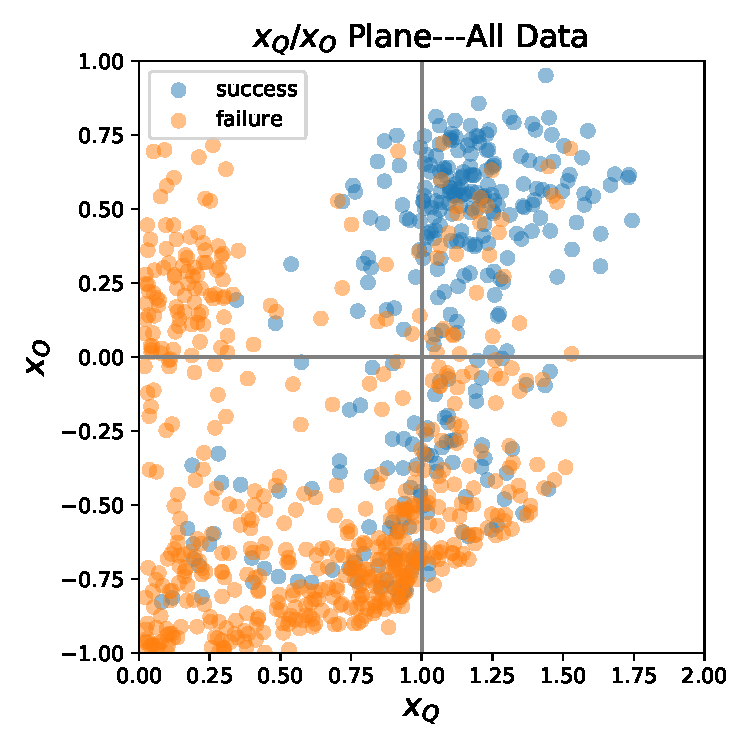
\includegraphics[width=0.7\linewidth]{Figures/xQxO_Plane.pdf}
        \vfill
        \caption{Total set of generated networks}
        \label{fig:tot_set}
    \end{subfigure}%
    \\
    % \hfill
    \begin{subfigure}[b]{0.80\linewidth}
        \centering
        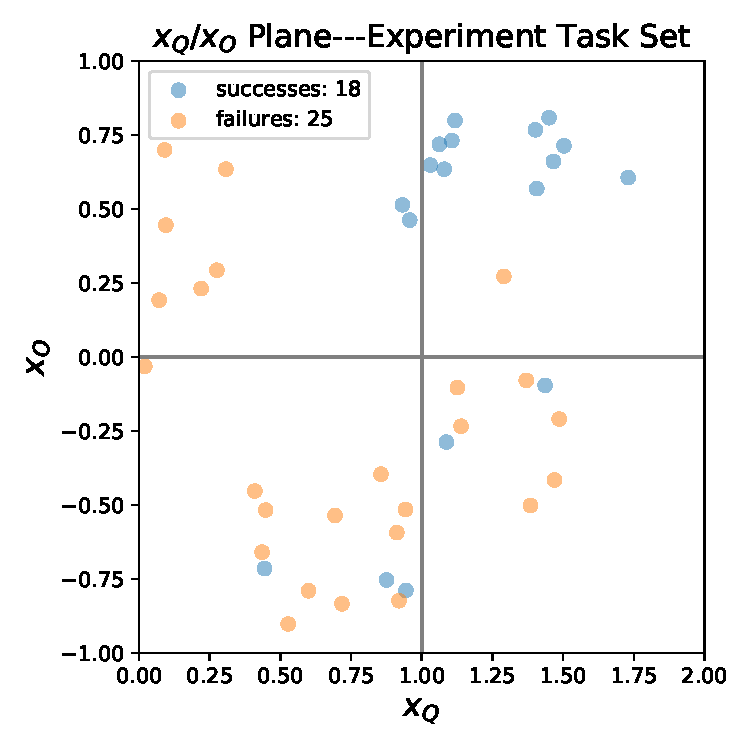
\includegraphics[width=0.7\linewidth]{Figures/xQxO_plane_experiment_set.pdf}
        \caption{Subset of networks used in the MTurk experiment}
        \label{fig:exp_set}
    \end{subfigure} 
    \caption{Example road networks. UGV starts at yellow, Pursuer beings at red, and the exit is green.}
    \label{fig:experiment_data}
    \vspace{-0.2cm}
\end{figure}

\brett{need some explanation about the coloring, and how we got that}
In order to understand the effects that the two \famsec{} factors had over the entire \xQ{}/\xO{} space, we selected the 43 examples from the full data set by splitting the space into grids and then proportionally selecting networks based on success and failure. First the data was split in quadrants and the total number of networks from each quadrant was selected based on the proportion of networks in the quadrant (in this case the proportion was [0.229,0.180,0.434,0.156] for quadrants 1-4 respectively, here quadrants start at 1 in the top right corner, 2 in the top left, et cetera).

For each quadrant the task set networks were chosen as follows: 1)calculate the total number of failures/successes based on the proportion of successes and failures in the same quadrant in the full data set; 2) draw successful networks in a pseudo-random way; 3) do the same as in 2) for the failure examples. The final counts in each quadrant are [12, 8, 15, 8], \brett{there was an artificial floor and maximum set on the number of examples in each quadrant, need to talk about that a little}.

\begin{tabular}{r|ccccc}
\toprule
             & Total & Quad. 1 & Quad. 2 & Quad. 3 & Quad. 4 \\ \hline
           N &    43 &      12 &       8 &      15 &       8 \\
  Proportion & 1.000 &   0.229 &   0.180 &   0.434 &   0.156 \\
   Successes &    18 &      11 &       2 &       3 &       2 \\
    Failures &    25 &       1 &       6 &      12 &       6 \\
Success/Fail &    -- &   9.714 &   0.283 &   0.214 &   0.417 \\
\bottomrule
\end{tabular}
